\textbf{1.1.} 把总电量为 $Q$ 的同一种电荷分成两部分，一部分均匀分布在地球上，另一部分均匀分布在月球上，使它们之间的库仑力正好抵消万有引力。已知 $1 / (4\pi \varepsilon_0) = 9.00 \times 10^9 \mathrm{~N} \cdot \mathrm{m}^2 \cdot \mathrm{C}^{-2}$ ，引力常数 $G = 6.67 \times 10^{-11} \mathrm{~N} \cdot \mathrm{m}^2 \cdot \mathrm{kg}^{-2}$ ，地球质量为 $5.98 \times 10^{24} \mathrm{~kg}$ ，月球质量为 $7.34 \times 10^{22} \mathrm{~kg}$ 。

(1) 求 Q 的最小值;

(2) 如果电荷分配与质量成正比, 求 Q.

\vfill

\textbf{1.2.} 真空中有一点电荷 $Q$ 固定不动, 另一质量为 $m$ 、电荷为 $-q$ 的质点, 在它们之间的库仑力的作用下, 绕 $Q$ 做匀速圆周运动, 半径为 $r$ , 周期为 $T$ . 证明

$$
\frac {r ^ {3}}{T ^ {2}} = \frac {q Q}{1 6 \pi^ {3} \varepsilon_ {0} m}
$$

\vfill

\newpage

\textbf{1.3.} 有三个点电荷,电量都是 $q = 1.6 \times 10^{-19} \mathrm{C}$ , 分别固定在边长为 $a = 3.0 \times 10^{-10} \mathrm{~m}$ 的正三角形三个顶点, 在这三角形中心 $O$ , 有一个质量为 $m = 2.3 \times 10^{-26} \mathrm{~kg}$ , 电量为 $Q = -4.8 \times 10^{-19} \mathrm{C}$ 的粒子.

(1) 证明: 这个粒子处在平衡位置(即作用在它上面的库仑力为零);

(2) 求这粒子以 O 为中心沿一轴线(该轴线过 O 并与三角形的平面互相垂直)做微小振动的频率 $\nu$ .

\vfill

\textbf{1.4.} 电量为 $Q$ 的两个点电荷，相距 $2l$ ，在其连线的中垂面上放一点电荷 $q_{0}$ ，求证该点电荷在中垂面上受力的极大值的轨迹是一个圆，并给出该圆的半径.

\vfill

\newpage

\textbf{1.5.} 习题1.5图中的 $q$ 和 $l$ 都已知，这样的四个点电荷称作平面电四极子。图中 $A$ 点与电四极子在同一平面内，它到电四极子中心 $O$ 的距离为 $x, AO$ 与正方形的两边平行。

(1) 求 A 点的电场强度 E;

(2) 当 $x \gg l$ 时, $\pmb{E} = ?$ .
\begin{center}
    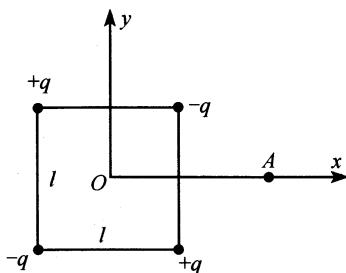
\includegraphics[width=0.3\linewidth]{figures/fig_1_5.jpg}
\end{center}

\vfill

\textbf{1.6.} 如习题 1.6 图所示, 电荷分布在半径为 R 的半圆环上, 线电荷密度为 $\lambda_{0}\sin\theta, \lambda_{0}$ 为常数, $\theta$ 为半径 OB 和直径 AC 间的夹角. 证明 AC 上任一点的电场强度都与 AC 垂直.
\begin{center}
    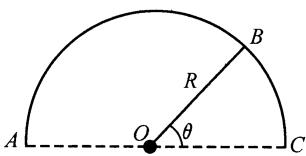
\includegraphics[width=0.3\linewidth]{figures/fig_1_7_1.jpg}
\end{center}
\vfill

\newpage

\textbf{1.7.} 一无限长均匀带电导线, 线电荷密度为 $\lambda$ , 一部分弯成半圆形, 其余部分为两条无穷长平行直导线, 两直线都与半圆的直径 $AB$ 垂直, 如习题 1.7 图所示, 求圆心 $O$ 处的电场强度.

\begin{center}
    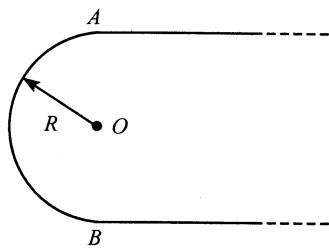
\includegraphics[width=0.3\linewidth]{figures/fig_1_7_2.jpg}
\end{center}

\vfill

\textbf{1.8.} 把电偶极矩为 $p = ql$ 的电偶极子放在点电荷 $Q$ 的电场内， $p$ 的中心 $O$ 到 $Q$ 的距离为 $D$ ，如习题 1.8 图所示。若 $p$ 分别 (1) 平行于 $OQ$ ; (2) 垂直于 $OQ$ ，求偶极子所受的力和力矩。
\begin{center}
    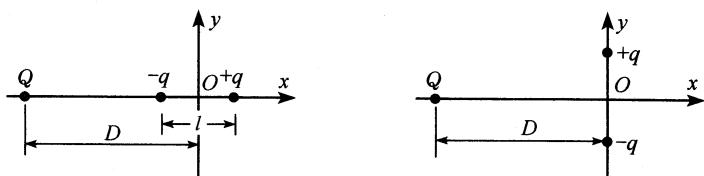
\includegraphics[width=0.6\linewidth]{figures/fig_1_8.jpg}
\end{center}

\vfill

\newpage

\textbf{1.9.} 有两个同心的均匀带电球面，内、外半径分别为 $R_{1}$ 和 $R_{2}$ ，外球面的电荷面密度为 $+\sigma$ ，球外各处的电场强度都是零，试求：

（1）内球面上的电荷面密度；

（2）两球面间离球心为 $r$ 处的电场强度 $\pmb{E}$ ；

（3）小球面内的电场强度 $\pmb{E}$ .

\vfill

\textbf{1.10.} 如习题 1.10 图所示,一厚度为 b 的无限大均匀带电板置于真空中,电荷体密度为 $\rho=kx(0\leqslant x\leqslant b)$ , 其中 k 是一正的常数,试求空间各点的电场强度.
\begin{center}
    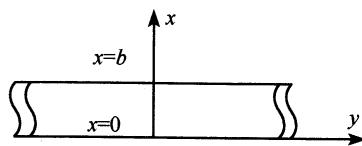
\includegraphics[width=0.3\linewidth]{figures/fig_1_11.jpg}
\end{center}
\vfill

\newpage

\textbf{1.11.} 根据量子力学, 氢原子在正常状态下核外电荷的分布如下: 离核心 r 处, 电荷的体密度 $\rho(r) = -qe^{-2r/a}/(\pi a^{3})$ , 式中 $q = 1.60 \times 10^{-19}C$ 是

核外电荷总量的绝对值, $a=5.29\times10^{-11}m$ 是玻尔半径.试求:

(1) 核外电荷的总电量；

(2) 核外电荷在 r 处的电场强度 E.


\vfill

\textbf{1.12.} 如习题 1.12 图所示, 空间有两个球, 球心间距离小于半径之和, 因此有一部分重叠 (见图). 今使一球充满密度为 $\rho$ 的均匀正电荷, 另一球充满密度为 $-\rho$ 的均匀负电荷, 以至于重叠区域无电荷. 求这重叠区域内的电场强度 $E$ , 说明 $E$ 是匀强电场.
\begin{center}
    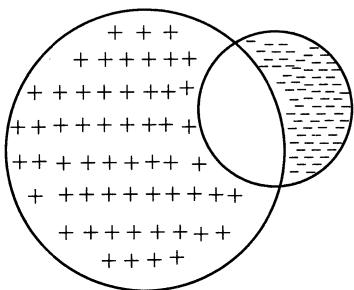
\includegraphics[width=0.3\linewidth]{figures/fig_1_13_1.jpg}
\end{center}
\vfill

\newpage

\textbf{1.13.} 在半导体 p-n 结附近总是堆积着正、负电荷，在 n 区内有正电荷，p 区内有负电荷，两区电荷的代数和为零。我们把 p-n 结看成一对带正、负电荷的无限大平板，它们相互接触（习题 1.13 图）。取 x 轴的原点在 p、n 区的交界面上，n 区的范围是 $-x_{n} \leqslant x \leqslant 0$ ，p 区的范围是 $0 \leqslant x \leqslant x_{p}$ 。设两区内电荷分布均匀，n 区电荷密度为 $N_{D}e$ ，p 区电荷密度为 $-N_{A}e$ ，称为突变结模型. 设 $N_{D}$ 、 $N_{A}$ 是常数，且 $N_{A}x_{p}=N_{D}x_{n}$ ，证明电场的分布为

(1) n 区: $E(x)=N_{\mathrm{D}}e(x_{\mathrm{n}}+x)/\varepsilon_{0}$ ;

(2) p 区: $E(x)=N_{\mathrm{A}}e(x_{\mathrm{p}}-x)/\varepsilon_{0}$ .

\begin{center}
    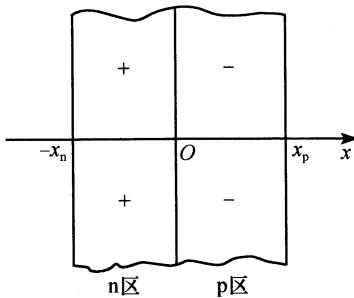
\includegraphics[width=0.3\linewidth]{figures/fig_1_13_2.jpg}
\end{center}

\vfill

\textbf{1.14.} 设气体放电形成的等离子体圆柱内的体电荷分布可表为 $\rho_{\mathrm{e}}(r) = \rho_0[1 + (r / a)^2 ]^{-2}$ , $r$ 是到其对称轴的距离, $\rho_0$ 是轴线上的电荷密度, $a$ 是常数, 求电场分布.

\vfill

\newpage

\textbf{1.15.} 如习题 1.15 图所示, AB=2l, 弧 OCD 是以 B 为中心, l 为半径的半圆. A 点有正电荷 +q, B 点有负电荷 -q.

(1) 把正电荷 Q 从 O 点沿弧 OCD 移到 D 点, 电场力对它做了多少功?

(2) 把负电荷 -Q 从 D 点沿 AB 延长线移到无穷远处, 电场力对它做了多少功?
\begin{center}
    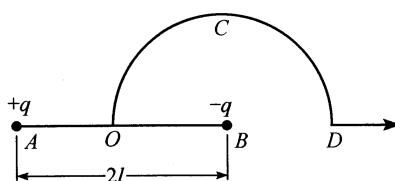
\includegraphics[width=0.3\linewidth]{figures/fig_1_15.jpg}
\end{center}

\vfill

\textbf{1.16.} 证明: 在无电荷分布的静电场中, 凡是电场线都是平行直线的地方, 电场强度的大小必定处处相等. 换句话说, 凡是电场强度的方向处处相同的地方, 电场强度的大小必定处处相等. (提示: 利用高斯定理和环路定理, 分别证明沿同一电场线和不同电场线上任意两点的场强相等.)

\vfill

\newpage

\textbf{1.17.} 线电四极子如习题 1.17 图所示, 求它在 $r \gg l$ 处的点 $A(r, \theta)$ 处所产生的电势 $U$ 和电场强度 $\pmb{E}$ .
\begin{center}
    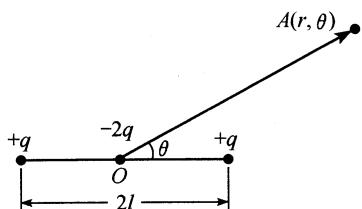
\includegraphics[width=0.3\linewidth]{figures/fig_1_17_1.jpg}
\end{center}
\vfill

\textbf{1.18} 面电四极子如习题 1.18 图所示, 点 $A(r, \theta)$ 与四极子共面, 极轴 $(\theta = 0)$ 通过正方形中心并与两边平行. 设 $r \gg l$ , 求面电四极子在点 $A$ 处产生的电势和电场强度.

\begin{center}
    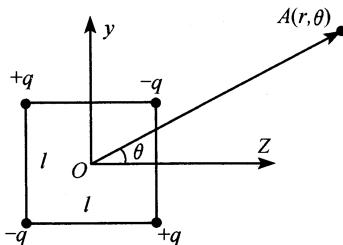
\includegraphics[width=0.3\linewidth]{figures/fig_1_17_2.jpg}
\end{center}

\vfill
\newpage

\textbf{1.19.} 两均匀带电的无限长直轴圆筒，内筒半径为 a，沿轴线单位长度的电量为 $\lambda_{c}$ ，外筒半径为 b，沿轴线单位长度的电量为 $-\lambda_{c}$ 。试求：

(1) 离轴线为 r 处的电势 U;

(2) 两筒的电势差.

\vfill



\textbf{1.20.} 设氢原子处于基态时的核外电荷呈球对称分布，其电荷密度为： $\rho(r)=-qe^{-2r/a}/(\pi a^{3})$ ，r为离核的距离，q为电子电荷的大小，a是玻尔半径。求在r处

(1) 核外电荷产生的电势；

(2) 所有电荷产生的电势.

\vfill
\newpage

\textbf{1.21} 两个均匀带电的圆面共轴线, 半径都为 $R$ , 相距为 $l$ , 电荷面密度分别为 $+\sigma$ 和 $-\sigma$ , 它们间轴线的中点为原点 $O$ , 沿轴线取为 $x$ 轴, 如习题 1.21 图所示. 已知 $l \ll R$ , 试求轴线上 $x$ 处的电势和电场强度.

\begin{center}
    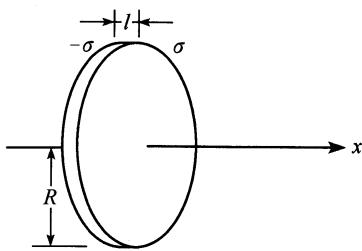
\includegraphics[width=0.3\linewidth]{figures/fig_1_20.jpg}
\end{center}

\vfill
\newpage
